% Usage: knitr slide

%
%### One sample/Paired: Modification of Student's sleep data ###%
%
%d1 <- sleep$extra[sleep$group==2] - sleep$extra[sleep$group==1]
%d1[1] <- d1[1] * -1

\chapter{Nonparametric Statistical Tests}\label{chap:nonpar}\ros{9}\katz{5.4}
\section{When to use non-parametric methods}
\bi
\item Short answer: Good default when $P$-values are needed
\item Nonparametric methods are those not requiring one to assume a
  certain distribution for the raw data
  \bi
  \item In contrast, parametric methods assume data come from some underlying distribution
  \item $t$-tests assume the data come form a Normal distribution with parameters $\mu$ and $\sigma^2$ for the mean and variance, respectively
  \ei
\item Response variable ordinal or interval
\item For ordinal responses nonparametric methods are preferred
  because they assume no spacing between categories
\item No problem in using nonparametric tests on interval data
 \bi
 \item if normality holds, nonpar.\ test 0.95 efficient, i.e., has
   about the same power as the parametric test done on 0.95 of the
   observations\footnote{The large-sample efficiency of the Wilcoxon
     and Spearman tests compared to $t$ and $r$ tests is
     $\frac{3}{\pi} = 0.9549$.}
 \item if normality does not hold, nonpar.\ tests can be arbitrarily
   more efficient and powerful than the corresponding parametric test 
 \item an elegant and non-arbitrary way to deal with extreme values or
   outliers
 \item rank-based nonparametric tests give the analyst freedom from
   having to choose the correct transformation of the measurement (as
   long as the optimum transformation is monotonic)
 \ei
\item Nonparametric methods are robust, many parametric methods are
  not
 \bi
 \item Example: $t$-test comparing two sets of measurements\\
   1 2 3 4 5 6 7 8 9 10 \hfill vs.\ \hfill 7 8 9 10 11 12 13 14 15 16
   17 18 19 20\\
   means: 5.5 and 13.5, $P=0.000019$\\
   1 2 3 4 5 6 7 8 9 10 \hfill vs.\ \hfill 7 8 9 10 11 12 13 14 15 16
   17 18 19 20 \textbf{200}\\
   means: 5.5 and 25.9, $P=0.12$\\
   The SD is a particularly non-robust statistical estimator.
  \ei

\item Example: Fecal calprotectin being evaluated as a possible
  biomarker of disease severity (Figure \ref{fig:nonpar-calpro})
 \bi 
  \item Calprotectin has an upper detection limit
  \item Median can be calculated (mean cannot)
 \ei
\item If all you want is a $P$-value nonpar.\ tests are preferred
 \bi
 \item Especially if response is univariate and no need to adjust for
   covariates
 \ei
\item Pre-testing for normality and deciding nonparametric
  vs.\ parametric analysis is a bad idea
 \bi
 \item Tests for normality do not have a power of 1.0 and type I error
   of 0.0
 \item Leads to temptation, e.g., an investigator might ``forget'' to do the
   test of normality if the $t$-test is significant
 \item Doesn't acknowledge that nonparametric tests are very efficient
   even under normality
 \ei
\item A drawback is that nonpar.\ tests do not correspond to
  usual confidence limits for effects
 \bi
  \item E.g., a CL for the difference in 2 means may include zero whereas
  the Wilcoxon test yields $P=0.01$
  \item Point estimate that exactly corresponds to the Wilcoxon
    two-sample test is the Hodges-Lehman estimate of the location
    difference
  \bi
  \item median of all possible differences between a measurement from
    group 1 and a measurement from group 2
  \ei
 \ei
\item Nonparametric tests are often obtained by replacing the data
  with ranks across subjects and then doing the parametric test
\item Many nonpar.\ tests give the same $P$-value regardless of how
  the data are transformed; a careful choice of transformation (e.g.,
  log) must sometimes be used in the context of parametric tests
\item $P$-values computed using e.g.\ the $t$ distribution are quite
  accurate for nonparametric tests
\item In case of ties, midranks are used, e.g., if the raw data were
  105 120 120 121 the ranks would be 1 2.5 2.5 4

\begin{center}
\begin{tabular}{ll} \hline
Parametric Test & Nonparametric Counterpart \\ \hline
1-sample $t$    & Wilcoxon signed-rank \\
2-sample $t$    & Wilcoxon 2-sample rank-sum \\
$k$-sample ANOVA           & Kruskal-Wallis \\
Pearson $r$     & Spearman $\rho$ \\ \hline
\end{tabular}\end{center}
\ei

\section{One Sample Test: Wilcoxon Signed-Rank} \ros{9.3}\katz{5.10.E}
\bi
\item Almost always used on paired data where the column of values
  represents differences (e.g., post-pre) or log ratios
\item The \emph{sign test} is the simplest test for the median
  difference being zero in the population
 \bi
 \item it just counts the number of positive differences after tossing
   out zero differences
 \item tests $H_{0}:$Prob$[x>0]=\frac{1}{2}$, i.e., that it is
   equally likely in the population to have a value below zero as it
   is to have a value above zero
 \item this is the same as testing that the population median
   difference is zero
 \item as it ignores magnitudes completely, the test is inefficient
 \ei
\item In the Wilcoxon signed rank one-sample test, ranks of absolute
  differences are given the sign of the original difference
\item Magnitudes of raw data matter more here than with the Wilcoxon
  2-sample test
\item Observations with zero differences are ignored

\item Example: A crossover study in which the treatment order is  randomized \\
  Data arranged so that treatment A is in the first column, no matter which order treatment A was given


\begin{center}
\begin{tabular}{ccccc} \hline
A & B & B-A & Rank $|\mathrm{B-A}|$ & Signed Rank \\ \hline
5 & 6 & ~1 & 1.5 & ~1.5 \\
6 & 5 & -1 & 1.5 & -1.5 \\
4 & 9 & ~5 & 4.0 & ~4.0 \\
7 & 9 & ~2 & 3.0 & ~3.0 \\ \hline
\end{tabular}\end{center}

\item A good approximation to an exact $P$-value may be obtained by computing
\beq
z = \frac{\sum{SR_{i}}}{\sqrt{\sum{SR_{i}^{2}}}},
\eeq
where the signed rank for observation $i$ is $SR_{i}$.  This formula
already takes ties into account without using Rosner's messy Eq.\
9.5.  We look up $|z|$ against the normal distribution.  Here
$z=\frac{7}{\sqrt{29.5}}=1.29$ and and the 2-tailed $P$-value is given below.
\begin{Schunk}
\begin{Sinput}
sr <- c(1.5, -1.5, 4, 3)
z <- sum(sr) / sqrt(sum(sr ^ 2))
pval <- 2 * (1 - pnorm(abs(z)))
c(z=z, pval=pval)
\end{Sinput}
\begin{Soutput}
        z      pval 
1.2888045 0.1974661 
\end{Soutput}
\end{Schunk}
\item If all differences are positive or all are negative, the exact
  2-tailed $P$-value is $\frac{1}{2^{n-1}}$
 \bi
 \item implies that $n$ must exceed 5 for any possibility of
   significance at the $\alpha=0.05$ level for a 2-tailed test
 \ei
\ei

\subsection{One sample/Paired Test Example}

\bi
\item Sleep Dataset
\bi
\item Compare the effects of two soporific drugs.
\item Each subject receives placebo, Drug 1, and Drug 2
\item Study question: Is Drug 1 or Drug 2 more effective at increasing sleep?
\item Dependent variable: Difference in hours of sleep comparing Drug 2 to Drug 1
\item $H_0:$ For any given subject, the difference in hours of sleep is equally likely to be positive or negative
\item See P.~\pageref{sleeppaired} for a parametric test on these data
\ei
\ei
%\clearpage
\begin{table}[!hbp]
 \begin{center}
 \begin{tabular}{lrrrcc}\hline\hline
Subject & Drug 1 & Drug 2 & \color{red}Diff (2-1) & Sign & Rank \\ \hline
1  &$ 0.7$&$ 1.9$&$\color{red}1.2$&+&$3$\\
2  &$-1.6$&$ 0.8$&$\color{red}2.4$&+&$8$\\
3  &$-0.2$&$ 1.1$&$\color{red}1.3$&+&$4.5$\\
4  &$-1.2$&$ 0.1$&$\color{red}1.3$&+&$4.5$\\
5  &$-0.1$&$-0.1$&$\color{red}0.0$&NA&\\
6  &$ 3.4$&$ 4.4$&$\color{red}1.0$&+&$2$\\
7  &$ 3.7$&$ 5.5$&$\color{red}1.8$&+&$7$\\
8  &$ 0.8$&$ 1.6$&$\color{red}0.8$&+&$1$\\
9  &$ 0.0$&$ 4.6$&$\color{red}4.6$&+&$9$\\
10 &$ 2.0$&$ 3.4$&$\color{red}1.4$&+&$6$\\
\hline
\end{tabular}
\caption{Hours of extra sleep on drugs 1 and 2, differences, signs and
  signed ranks of sleep study data}
\end{center}
\end{table}
\begin{Schunk}
\begin{Sinput}
drug1 <- c(.7, -1.6, -.2, -1.2, -.1, 3.4, 3.7, .8, 0, 2)
drug2 <- c(1.9, .8, 1.1, .1, -.1, 4.4, 5.5, 1.6, 4.6, 3.4)
wilcox.test(drug2, drug1, paired=TRUE)
\end{Sinput}
\begin{Soutput}

	Wilcoxon signed rank test with continuity correction

data:  drug2 and drug1
V = 45, p-value = 0.009091
alternative hypothesis: true location shift is not equal to 0
\end{Soutput}
\begin{Sinput}
wilcox.test(drug2 - drug1)
\end{Sinput}
\begin{Soutput}

	Wilcoxon signed rank test with continuity correction

data:  drug2 - drug1
V = 45, p-value = 0.009091
alternative hypothesis: true location is not equal to 0
\end{Soutput}
\begin{Sinput}
wilcox.test(drug2 - drug1, correct=FALSE)
\end{Sinput}
\begin{Soutput}

	Wilcoxon signed rank test

data:  drug2 - drug1
V = 45, p-value = 0.007632
alternative hypothesis: true location is not equal to 0
\end{Soutput}
\begin{Sinput}
sr <- c(3, 8, 4.5, 4.5, 0, 2, 7, 1, 9, 6)
z <- sum(sr) / sqrt(sum(sr ^ 2))
c(z=z, pval=2 * (1 - pnorm(abs(z))))
\end{Sinput}
\begin{Soutput}
          z        pval 
2.667911250 0.007632442 
\end{Soutput}
\begin{Sinput}
d <- data.frame(Drug=c(rep('Drug 1', 10), rep('Drug 2', 10),
                  rep('Difference', 10)),
                extra=c(drug1, drug2, drug2 - drug1))
\end{Sinput}
\end{Schunk}
\bi 
\item Interpretation: Reject $H_0$, Drug 2 increases sleep by the same hours as Drug 1 ($p = 0.008$)
\item Could also perform sign test on sleep data
 \bi
 \item If drugs are equally effective, should have same number of `+' and '-'
 \item Observed data: 0 `-', 9 `+', throw out 1 `no change' 
 \item Sign test (2-sided) $P$-value: Probability of observing 9 of 9
   + or 9 of 9 -
 \item $p = 0.004$, so evidence against $H_0$
 \ei
\ei
\begin{Schunk}
\begin{Sinput}
2 * (1 / 2) ^ 9    # 2 * to make it two-tailed
\end{Sinput}
\begin{Soutput}
[1] 0.00390625
\end{Soutput}
\end{Schunk}

\bi
\item The signed rank test assumes that the distribution of differences is
  symmetric
\item When the distribution is symmetric, the signed rank test tests whether the
  median difference is zero
\item In general it tests that, for two randomly chosen observations
  $i$ and $j$ with values (differences) $x_i$ and $x_j$, that the
  probability that $x_{i}+x_{j} > 0$ is $\frac{1}{2}$
\item The estimator that corresponds exactly to the test in all
  situations is the pseudomedian, the median of all possible pairwise
  averages of $x_i$ and $x_j$, so one could say that the signed rank
  test tests $H_{0}$: pseudomedian=0
\item The value $\frac{\overline{SR}}{n+1}-\frac{1}{2}$ estimates the
  probability that two randomly chosen observations have a positive
  sum, where $\overline{SR}$ is the mean of the column of signed ranks
\item To test $H_{0}:\eta=\eta_{0}$, where $\eta$ is the population median
  (not a difference) and $\eta_{0}$ is some constant, we create the $n$ values
  $x_{i} - \eta_{0}$ and feed those to the signed rank test, assuming
  the distribution is symmetric
\item When all nonzero values are of the same sign, the test reduces
  to the \emph{sign test} and the 2-tailed $P$-value is
  $(\frac{1}{2})^{n-1}$ where $n$ is the number of nonzero values
\ei

Test whether the continuity correction makes $P$-values closer to the
exact calculation\footnote{The exact $P$-value is available only when
  there are no ties.}, and compare to our simple formula.
\begin{Schunk}
\begin{Sinput}
# Assume we are already starting with signed ranks as x
wsr <- function(x, ...) wilcox.test(x, ...)$p.value
sim <- function(x) {
  z <- sum(x) / sqrt(sum(x ^ 2))
  2 * (1 - pnorm(abs(z))) }
all <- function(x) round(c(
  continuity=wsr(x, correct=TRUE, exact=FALSE),
  nocontinuity=wsr(x, correct=FALSE, exact=FALSE),
  exact=wsr(x, exact=TRUE),
  simple=sim(x)), 4)
all(1:4)
\end{Sinput}
\begin{Soutput}
  continuity nocontinuity        exact       simple 
      0.1003       0.0679       0.1250       0.0679 
\end{Soutput}
\begin{Sinput}
all(c(-1, 2 : 4))
\end{Sinput}
\begin{Soutput}
  continuity nocontinuity        exact       simple 
      0.2012       0.1441       0.2500       0.1441 
\end{Soutput}
\begin{Sinput}
all(c(-2, c(1, 3, 4)))
\end{Sinput}
\begin{Soutput}
  continuity nocontinuity        exact       simple 
      0.3613       0.2733       0.3750       0.2733 
\end{Soutput}
\begin{Sinput}
all(c(-1, -2, 3 : 5))
\end{Sinput}
\begin{Soutput}
  continuity nocontinuity        exact       simple 
      0.2807       0.2249       0.3125       0.2249 
\end{Soutput}
\begin{Sinput}
all(c(-5, -1, 2, 3, 4, 6))
\end{Sinput}
\begin{Soutput}
  continuity nocontinuity        exact       simple 
      0.4017       0.3454       0.4375       0.3454 
\end{Soutput}
\end{Schunk}
From these examples the guidance is to:
\bi
\item Use the exact calculation if there are no ties
\item Otherwise use the continuity correction (i.e., the default in
  \Co{wilcox.test}) unlike the recommendation for the Pearson $\chi^2$ test
\ei

\section{Two Sample Test: Wilcoxon--Mann--Whitney} \ros{9.4}\katz{5.5.B}
\bi
\item The Wilcoxon--Mann--Whitney (WMW) 2-sample rank sum test is for
  testing for equality of central tendency of two distributions (for
  unpaired data)
\item Ranking is done by combining the two samples and ignoring which
  sample each observation came from
\item Example:

\begin{center}\begin{tabular}{lrrrr} \hline
Females           & 120 & 118 & 121 & 119 \\
Males             & 124 & 120 & 133 &     \\ \hline
Ranks for Females & 3.5 & ~~1 & ~~5 & ~~2 \\
Ranks for Males   & ~~6 & 3.5 & ~~7 &     \\ \hline
\end{tabular}\end{center}

\item Doing a 2-sample $t$-test using these ranks as if they were raw
  data and computing the $P$-value against 4+3-2=5 d.f.\ will work
  quite well
\item Some statistical packages compute $P$-values exactly (especially
  if there are no ties)
\item Loosely speaking the WMW test tests whether the population
  medians of the two groups are the same
\item More accurately and more generally, it tests whether
  observations in one population tend to be larger than observations
  in the other
\item Letting $x_1$ and $x_2$ respectively be randomly chosen
  observations from populations one and two, WMW tests
  $H_{0}:c=\frac{1}{2}$, where $c=$Prob$[x_{1} > x_{2}]$
\item The $c$ index (\emph{concordance probability}) may be estimated
  by computing
\beq
C = \frac{\bar{R}-\frac{n_{1}+1}{2}}{n_{2}},
\eeq
where $\bar{R}$ is the mean of the ranks in group 1; \\
For the above data $\bar{R} = 2.875$ and
$c=\frac{2.875-2.5}{3}=0.125$, so we estimate that the probability is
0.125 that a randomly chosen female has a value greater than a randomly
chosen male.
\item In diagnostic studies where $x$ is the continuous result of a
  medical test and the grouping variable is diseased vs.\ nondiseased,
  $c$ is the area under the receiver operating characteristic (ROC) curve
\item Test still has the ``probability of ordering'' interpretation
  when the variances of the two samples are markedly different, but it
  no longer tests anything like the difference in population medians
\ei
If there is no overlap between measurements from group 1 and those
from group 2, the exact 2-sided $P$-value for the Wilcoxon test is $2
/ \frac{n!}{n_{1}! n_{2}!}$.  If $n_{1}=n_{2}$, $n_{1}$ must be $\geq
4$ to obtain $P < 0.05$ (in this case $P = 0.029$). 
% Thanks: Rameela and Bill
%If R1 denotes the rank sum of the group with sample size m, then the
%smallest possible value of R1 is the sum of the m smallest ranks 1 + 2 +
%... m = m*(m+1)/2. The probability of this value is 1/[(m+n)Cm] -- C
%implies choose.

\subsection{Two sample WMW example}
\bi 
\item Fecal calprotectin being evaluated as a possible biomarker of
  disease severity 
\item Calprotectin measured in 26 subjects, 8 observed to have no/mild
  activity by endoscopy 
\item Calprotectin has upper detection limit at 2500 units
 \bi 
 \item A type of missing data, but need to keep in analysis
 \ei
\item Study question: Are calprotectin levels different in subjects
  with no or mild activity compared to subjects with moderate or
  severe activity? 
\item Statement of the null hypothesis
 \bi 
 \item $H_0:$ Populations with no/mild activity have the same
   distribution of calprotectin as populations with moderate/severe
   activity 
 \item $H_0: C = \frac{1}{2}$
 \ei
\ei
\begin{Schunk}
\begin{Sinput}
#Fecal Calprotectin: 2500 is above detection limit
calpro <- c(2500, 244, 2500, 726, 86, 2500, 61, 392, 2500, 114, 1226,
            2500, 168, 910, 627, 2500, 781, 57, 483, 30, 925, 1027,
            2500, 2500, 38, 18)

# Endoscopy score: 1 = No/Mild, 2=Mod/Severe Disease
# Would have been far better to code dose as 4 ordinal levels
endo <- c(2, 1, 2, 2, 2, 1, 1, 2, 2, 1, 2, 2, 1, 2, 2, 2, 2, 1, 2,
          2, 2, 2, 2, 2, 1, 1)
endo <- factor(endo, 1 : 2,
               c("No or Mild Activity", "Moderate or Severe Activity"))
require(ggplot2)   # Fig. (*\ref{fig:nonpar-calpro}*)
ggplot(data.frame(endo, calpro), aes(y=calpro, x=endo)) +
  geom_boxplot(color='lightblue', alpha=.85, width=.4) +
  geom_dotplot(binaxis='y', stackdir='center', position='dodge') +
    xlab('') + ylab('Fecal Calprotectin') + coord_flip() +
      geom_hline(aes(yintercept=2500, col='red'), linetype='dotted')
\end{Sinput}
\begin{Sinput}
wilcox.test(calpro ~ endo)
\end{Sinput}
\begin{Soutput}

	Wilcoxon rank sum test with continuity correction

data:  calpro by endo
W = 23.5, p-value = 0.006814
alternative hypothesis: true location shift is not equal to 0
\end{Soutput}
\begin{figure}[htbp]

\centerline{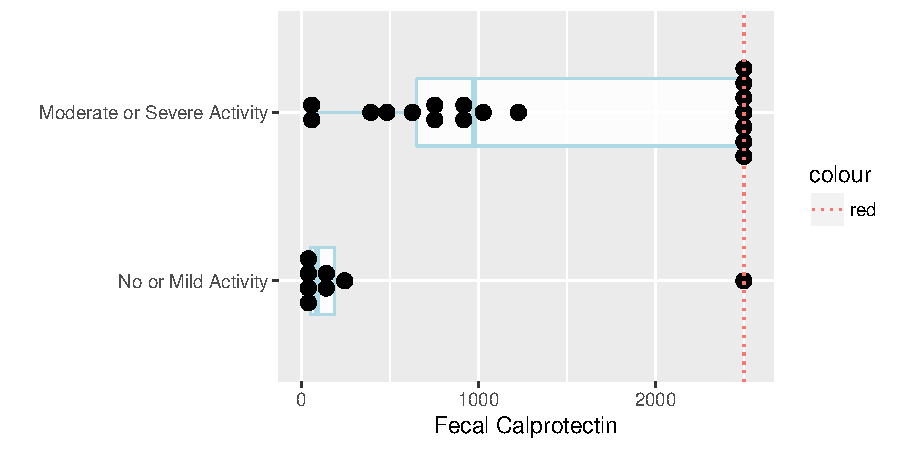
\includegraphics{nonpar-calpro-1} }

\caption[Fecal calprotectin by severity]{Fecal calprotectin by endoscopy severity rating. Red dotted line is the detection limit.  Ordinal disease categories should not have been combined.}\label{fig:nonpar-calpro}
\end{figure}
\end{Schunk}
% See http://docs.ggplot2.org/0.9.3/geom_dotplot.html
The following plots the ranks that are used in the
Wilcoxon-Mann-Whitney two-sample ranksum test.
\begin{Schunk}
\begin{Sinput}
ggplot(data.frame(endo, calpro), aes(y=rank(calpro), x=endo)) + #Fig (*\ref{fig:nonpar-calpror}*)
  geom_dotplot(binaxis='y', stackdir='center', position='dodge') +
    xlab('') + ylab('Rank of Fecal Calprotectin') + coord_flip()
\end{Sinput}
\begin{figure}[htbp]

\centerline{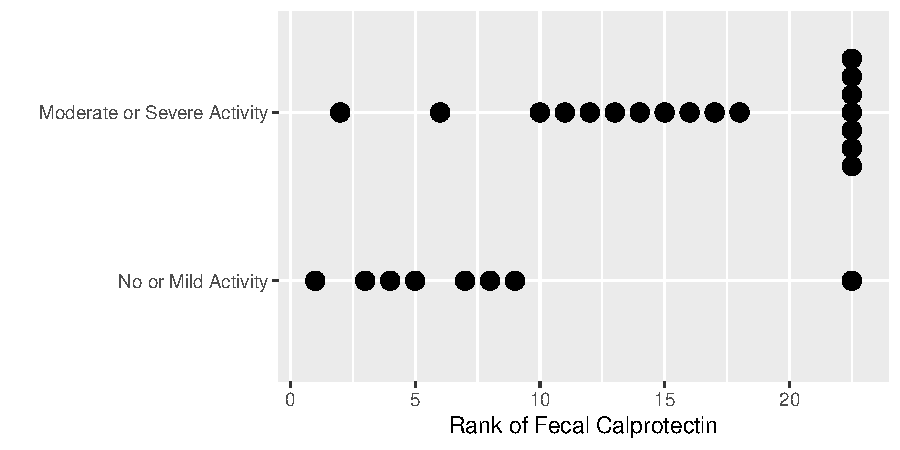
\includegraphics{nonpar-calpror-1} }

\caption[Ranks of calprotectin]{Ranks of calprotectin}\label{fig:nonpar-calpror}
\end{figure}
\end{Schunk}
\bi
\item Test statistic $W$ equals the sum of the ranks in the no/mild group minus $n_1 * (n_1 + 1) / 2$, where $n_1$ is the number of subjects in then no/mild sample
\item $W = 59.5 - \frac{8*9}{2} = 23.5$
\item A common (but loose) interpretation: People with moderate/severe activity have higher \textit{median} fecal calprotectin levels than people with no/mild activity ($p = 0.007$).
\item Better: remove \textit{median} and supplement with the $c$-index
  (concordance probability) or Somers' $D_{xy}$ rank correlation
  between calprotectin and endoscopy status.  The code for the \R\
  \Co{somers2} function shows how the concordance probability is
  computed from the mean of the ranks in one of the two groups.
\ei
\begin{Schunk}
\begin{Sinput}
require(Hmisc)
# Convert endo to a binary variable
somers2(calpro, endo=='Moderate or Severe Activity')
\end{Sinput}
\begin{Soutput}
         C        Dxy          n    Missing 
 0.8368056  0.6736111 26.0000000  0.0000000 
\end{Soutput}
\end{Schunk}
If you type \Co{somers2} to list the code for the function you will
see that the $c$-index is tightly related to the Wilcoxon test when
you see this code:
\begin{Schunk}
\begin{Sinput}
mean.rank <- mean(rank(x)[y == 1])
c.index <- (mean.rank - (n1 + 1)/2) / (n - n1)
\end{Sinput}
\end{Schunk}

\subsection{Point and Interval Estimates for Wilcoxon Two-Sample Comparison}
As mentioned earlier, the effect estimate that is exactly consistent
with the Wilcoxon two-sample test is the robust Hodges-Lehman estimator---the
median of all possible differences between a measurement from group 1
and a measurement from group 2.  There is a confidence interval for
this estimator.
\bi
\item Assume data come from distributions with same shape and differ only in location
\item Consider a sample of 4 males and 3 females
\item Considers all possible differences between sample 1 and sample 2
\ei
\begin{center}\begin{tabular}{l|cccc} \hline \hline \label{pg:nonpar-mf}
 & \multicolumn{4}{c}{Female} \\
Male & 120 & 118 & 121 & 119 \\ \hline
124 & 4 & 6 & 3 & 5 \\ 
120 & 0 & 2 & -1 & 1 \\
133 & 13 & 15 & 12 & 14 \\ \hline
\end{tabular}\end{center}
\bi
\item Hodges-Lehman estimate of the sex effect: median of the 12
  differences = 4.5
\ei
\begin{Schunk}
\begin{Sinput}
female <- c(120, 118, 121, 119)
male   <- c(124, 120, 133)
differences <- outer(male, female, '-')
differences
\end{Sinput}
\begin{Soutput}
     [,1] [,2] [,3] [,4]
[1,]    4    6    3    5
[2,]    0    2   -1    1
[3,]   13   15   12   14
\end{Soutput}
\begin{Sinput}
median(differences)
\end{Sinput}
\begin{Soutput}
[1] 4.5
\end{Soutput}
\begin{Sinput}
wilcox.test(male, female, conf.int=TRUE)
\end{Sinput}
\begin{Soutput}

	Wilcoxon rank sum test with continuity correction

data:  male and female
W = 10.5, p-value = 0.1536
alternative hypothesis: true location shift is not equal to 0
95 percent confidence interval:
 -1 15
sample estimates:
difference in location 
              4.791134 
\end{Soutput}
\end{Schunk}
In general, $1 - \alpha$ confidence intervals are the set of values that if
hypothesized to be the true location parameter would not be rejected
at the $\alpha$ level.  \Co{wilcox.test} computes the location shift
by solving for the hypothesized value that yields $P=1.0$ instead of
the more proper median of all differences.  Look into this further by
plotting the $P$-value as a function of the hypothesized value.
\begin{Schunk}
\begin{Sinput}
dif  <- seq(-3, 15, by=.1)
n    <- length(dif)
pval <- numeric(n)
for(i in 1 : n) pval[i] <- wilcox.test(male - dif[i], female)$p.value
\end{Sinput}
\begin{Sinput}
ggplot(data.frame(dif, pval), aes(x=dif, y=pval)) +
  geom_step() +
  geom_hline(yintercept=.05, col='red', linetype='dotted') +
  geom_vline(xintercept=c(4.5, 4.791, -1, 15), col='red', linetype='dotted') +
  xlab('Difference') + ylab('P-value')
\end{Sinput}
\begin{figure}[htbp]

\centerline{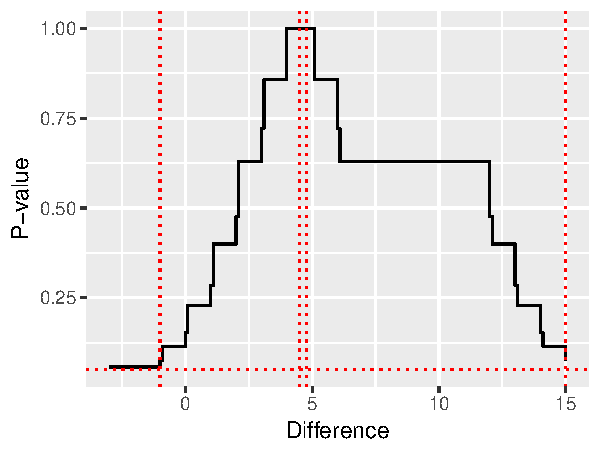
\includegraphics{nonpar-checkhl-1} }

\caption[Wilcoxon $P$-value vs.\ hypothesized difference.]{Wilcoxon $P$-value vs.\ hypothesized male-female difference.  Horizontal line is $P=0.05$.  Vertical lines from left to right are the lower 0.95 confidence limit from \Co{wilcox.test}, the median difference, the Hodges-Lehman estimator as computed by \Co{wilcox.test}, and the upper 0.95 confidence limit from \Co{wilcox.test}.}\label{fig:nonpar-checkhl}
\end{figure}
\end{Schunk}
See Section~\ref{sec:nonpar-clmed} for a more approximate confidence interval.

\section{Confidence Intervals for Medians and Their Differences} \altman{36-43}\label{sec:nonpar-clmed}
\bi 
\item Confidence intervals for the median (one sample)
\bi 
\item Table 18.4 (Altman) gives the ranks of the observations to be
  used to give approximate confidence intervals for the median 
\item e.g., if $n = 12$, the $3^\textrm{rd}$ and $10^\textrm{th}$
  largest values give a $0.961$ confidence interval 
\item For larger sample sizes, the lower ranked value ($r$) and upper
  ranked value ($s$) to select for an approximate $0.95$ confidence
  interval for the population median is 
\beq
r = \frac{n}{2} - 1.96*\frac{\sqrt{n}}{2} \hspace{.4cm}\textrm{and}
\hspace{.4cm} s = 1 + \frac{n}{2} + 1.96*\frac{\sqrt{n}}{2} 
\eeq
\item e.g., if $n = 100$ then $r = 40.2$ and $s = 60.8$, so we would pick the $40^\textrm{th}$ and $61^\textrm{st}$ largest values from the sample to specify a $0.95$ confidence interval for the population median
\item For exact confidence interval for the median see
  \href{https://stats.stackexchange.com/questions/186957}{here}, which
  also discusses why there is no exact nonparametric confidence
  interval for the mean.
\ei
\item Confidence intervals for the difference in two medians (two samples)
\bi
\item Assume data come from distributions with same shape and differ only in location
\item Considers all possibly differences between sample 1 and sample 2
  using male-female data on P.~\pageref{pg:nonpar-mf}
\item An estimate of the median difference (males - females) is the median of these 12 differences, with the $3^\textrm{rd}$ and $10^\textrm{th}$ largest values giving an (approximate) 0.95 CI
\item Median estimate = 4.5, 0.95 CI = [1, 13]
\item Specific formulas found in Altman, pages 40-41
\ei
\item Bootstrap \altman{159-163}
\bi
\item General method, not just for medians
\item Non-parametric, does not assume symmetry
\item Iterative method that repeatedly samples from the original data
\item Algorithm for creating a $0.95$ CI for the difference in two medians
\begin{enumerate}
\item Sample \textit{with replacement} from sample 1 and sample 2
\item Calculate the difference in medians, save result
\item Repeat Steps 1 and 2 1000 times
\end{enumerate}
\item A (naive) $0.95$ CI is given by the $25^\textrm{th}$ and $975^\textrm{th}$ largest values of your $1000$ median differences
\item For the male/female data, median estimate = 4.5, 0.95 CI = [-0.5, 14.5], which agrees with the conclusion from a WMW rank sum test ($p = 0.15$).
\ei
\ei
\begin{Schunk}
\begin{Sinput}
diffs <- numeric(1000)
set.seed(13)
for(i in 1 : 1000) diffs[i] <-
  median(sample(male, replace=TRUE)) - median(sample(female, replace=TRUE))
ggplot(data.frame(diffs), aes(x=diffs)) + xlab('Differences in Medians') +
  geom_histogram(bin_widith=.01, color='blue', fill='white')
\end{Sinput}
\begin{Sinput}
quantile(diffs, c(0.025, 0.975))
\end{Sinput}
\begin{Soutput}
 2.5% 97.5% 
 -0.5  14.5 
\end{Soutput}


\centerline{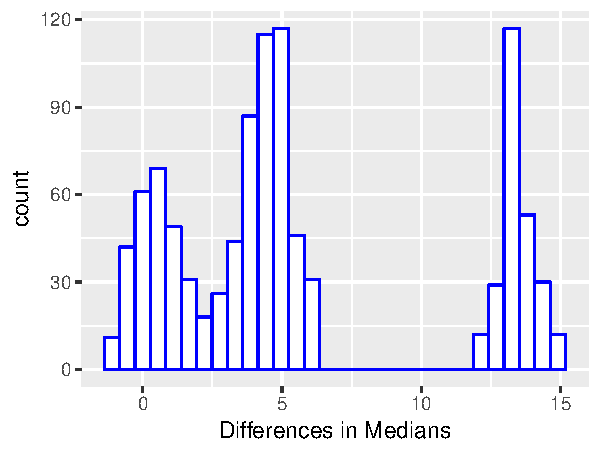
\includegraphics{nonpar-diffmedboot-1} }

\end{Schunk}
But recall that the Wilcoxon test does not really test the difference
in medians but rather the median of all differences.

\section{Strategy}
\bi
\item Don't assess normality of data
\item Use nonparametric test in any case, to get $P$-values
\item Use nonparametric confidence intervals for means and
  medians\footnote{A good nonparametric confidence for a population
    mean that does not even assume a symmetric distribution can be
    obtained from the bootstrap simulation procedure.}
  which will be more in conformance to what the nonpar.\ test is
  testing
\item To obtain nonparametric confidence limits for means and
  differences in means, the bootstrap percentile method may easily be
  used and it does not assume symmetry of the data distribution
\ei

\section{Generalizations}
The proportional odds ordinal logistic model is a generalization of
the Wilcoxon 2-sample and Kruskal-Wallis tests.  It can adjust for
covariates and estimate quantiles and mean responses.  There are other
ordinal response models that may fit better in certain cases, e.g.,
the Cox proportional hazards model.
